\documentclass{article}

\usepackage{hyperref}

\title{Package \textbf{CompSign}}
\author{Lena Morrill}
\date{October 2017}

\begin{document}

\maketitle

\textbf{CompSign} is a package for yadayada... overlooked that mutational signatures are compositional in nature yadayada. The reference manual can be found \href{https://github.com/lm687/CompSign/blob/master/CompSign.pdf}{here}.

\begin{knitrout}
\definecolor{shadecolor}{rgb}{0.969, 0.969, 0.969}\color{fgcolor}\begin{kframe}
\begin{alltt}
\hlstd{knitr}\hlopt{::}\hlstd{opts_chunk}\hlopt{$}\hlkwd{set}\hlstd{(}\hlkwc{cache} \hlstd{=} \hlnum{TRUE}\hlstd{)}
\end{alltt}
\end{kframe}
\end{knitrout}

\begin{knitrout}
\definecolor{shadecolor}{rgb}{0.969, 0.969, 0.969}\color{fgcolor}\begin{kframe}
\begin{alltt}
\hlcom{## This chunk was last ran in}
\hlkwd{timestamp}\hlstd{()}
\end{alltt}
\begin{verbatim}
## ##------ Tue Oct 23 16:07:05 2018 ------##
\end{verbatim}
\begin{alltt}
\hlcom{## install latest version}
\hlkwd{library}\hlstd{(devtools)}
\hlstd{devtools}\hlopt{::}\hlkwd{install_github}\hlstd{(}\hlstr{"lm687/CompSign"}\hlstd{)}
\end{alltt}


{\ttfamily\noindent\itshape\color{messagecolor}{\#\# Downloading GitHub repo lm687/CompSign@master}}\begin{verbatim}
## Rfast      (1.9.0  -> 1.9.1 ) [CRAN]
## rlang      (0.2.2  -> 0.3.0 ) [CRAN]
## robustbase (0.93-1 -> 0.93-3) [CRAN]
\end{verbatim}


{\ttfamily\noindent\itshape\color{messagecolor}{\#\# Installing 3 packages: Rfast, rlang, robustbase}}\begin{verbatim}
## 
##   There are binary versions available but the source versions are
##   later:
##              binary source needs_compilation
## Rfast         1.9.0  1.9.1              TRUE
## rlang         0.2.2  0.3.0              TRUE
## robustbase 0.93-1.1 0.93-3              TRUE
\end{verbatim}


{\ttfamily\noindent\itshape\color{messagecolor}{\#\# installing the source packages 'Rfast', 'rlang', 'robustbase'}}

{\ttfamily\noindent\bfseries\color{errorcolor}{\#\# Error in i.p(...): (converted from warning) installation of package 'Rfast' had non-zero exit status}}\begin{alltt}
\hlkwd{library}\hlstd{(CompSign)}
\hlkwd{library}\hlstd{(compositions)}
\end{alltt}
\end{kframe}
\end{knitrout}

\begin{knitrout}
\definecolor{shadecolor}{rgb}{0.969, 0.969, 0.969}\color{fgcolor}\begin{kframe}
\begin{alltt}
\hlcom{## This chunk was last ran in}
\hlkwd{timestamp}\hlstd{()}
\end{alltt}
\begin{verbatim}
## ##------ Tue Oct 23 16:07:17 2018 ------##
\end{verbatim}
\begin{alltt}
\hlcom{##########################}
\hlcom{####### Dummy data #######}
\hlcom{##########################}

\hlcom{### Example of matrix transformed into sign object}
\hlstd{input_dummy} \hlkwb{<-} \hlkwd{matrix}\hlstd{(}\hlkwd{runif}\hlstd{(}\hlnum{100}\hlstd{),} \hlnum{4}\hlstd{)}
\hlkwd{colnames}\hlstd{(input_dummy)} \hlkwb{<-} \hlkwd{paste0}\hlstd{(}\hlstr{'s'}\hlstd{,} \hlnum{1}\hlopt{:}\hlnum{25}\hlstd{);} \hlkwd{rownames}\hlstd{(input_dummy)} \hlkwb{<-} \hlkwd{paste0}\hlstd{(}\hlstr{'sam'}\hlstd{,} \hlnum{1}\hlopt{:}\hlnum{4}\hlstd{)}
\hlstd{sign_dummy} \hlkwb{<-} \hlkwd{to_sign}\hlstd{(input_dummy)}
\end{alltt}
\end{kframe}
\end{knitrout}

\section{Summarise the signature matrix}
\begin{knitrout}
\definecolor{shadecolor}{rgb}{0.969, 0.969, 0.969}\color{fgcolor}\begin{kframe}
\begin{alltt}
\hlcom{## This chunk was last ran in}
\hlkwd{timestamp}\hlstd{()}
\end{alltt}
\begin{verbatim}
## ##------ Tue Oct 23 16:07:17 2018 ------##
\end{verbatim}
\begin{alltt}
\hlkwd{add_together_matrix}\hlstd{(sign_dummy)}
\end{alltt}
\begin{verbatim}
## An object of class "sign"
## Slot "id":
## [1] "input_dummy"
## 
## Slot "id_samples":
## [1] "sam1" "sam2" "sam3" "sam4"
## 
## Slot "id_signatures":
##  [1] "s1"  "s2"  "s3"  "s4"  "s5"  "s6"  "s7"  "s8"  "s9"  "s10" "s11"
## [12] "s12" "s13" "s14" "s15" "s16" "s17" "s18" "s19" "s20" "s21" "s22"
## [23] "s23" "s24" "s25"
## 
## Slot "count_matrix":
##             s1        s2         s3         s4        s5        s6
## sam1 0.6233436 0.4169807 0.42993493 0.05794318 0.5901997 0.4031462
## sam2 0.3413632 0.9537744 0.40388599 0.77977055 0.3459038 0.6192916
## sam3 0.7667998 0.5407284 0.41226984 0.52461156 0.8846929 0.0349309
## sam4 0.2600229 0.1852972 0.08326648 0.72768078 0.4195605 0.2982445
##             s7         s8        s9       s10       s11       s12
## sam1 0.5173039 0.03627578 0.6358517 0.3560672 0.4794818 0.8603726
## sam2 0.9682418 0.51997587 0.5762934 0.9463702 0.4856246 0.6810569
## sam3 0.5646822 0.19521899 0.5881210 0.4894135 0.0917544 0.7878934
## sam4 0.7432367 0.24150709 0.7345787 0.9173480 0.3879061 0.6024034
##            s13        s14        s15       s16        s17        s18
## sam1 0.9625107 0.64921463 0.51214372 0.2608192 0.01568284 0.07549878
## sam2 0.4402104 0.59216471 0.54887152 0.3266606 0.35872920 0.54298686
## sam3 0.9492627 0.24655105 0.44548164 0.2954519 0.90683456 0.54280131
## sam4 0.3617747 0.08594473 0.04314753 0.5781598 0.24789950 0.09762706
##            s19       s20        s21       s22        s23       s24
## sam1 0.6848625 0.3172088 0.65449068 0.9566853 0.87854259 0.2507065
## sam2 0.4230498 0.4200921 0.20150530 0.3688930 0.44524506 0.4808561
## sam3 0.7456224 0.3255062 0.84818795 0.1185494 0.07345417 0.8769561
## sam4 0.2665278 0.1624959 0.05967938 0.7779736 0.45255367 0.5115345
##            s25
## sam1 0.2770414
## sam2 0.9197584
## sam3 0.5491871
## sam4 0.8128649
## 
## Slot "modified":
## [1] TRUE
\end{verbatim}
\begin{alltt}
\hlstd{results_sumarise} \hlkwb{<-} \hlkwd{summarise}\hlstd{(}\hlkwd{add_together_matrix}\hlstd{(sign_dummy))}
\hlstd{results_sumarise}\hlopt{$}\hlstd{General}
\end{alltt}
\begin{verbatim}
## [1] "Object of class sign"
\end{verbatim}
\end{kframe}
\end{knitrout}

\section{Linear model for numerical predictors}
\begin{knitrout}
\definecolor{shadecolor}{rgb}{0.969, 0.969, 0.969}\color{fgcolor}\begin{kframe}
\begin{alltt}
\hlcom{## This chunk was last ran in}
\hlkwd{timestamp}\hlstd{()}
\end{alltt}
\begin{verbatim}
## ##------ Tue Oct 23 16:07:17 2018 ------##
\end{verbatim}
\begin{alltt}
\hlstd{tmp_merged_compositional} \hlkwb{<-} \hlkwd{new}\hlstd{(}\hlstr{"merged_compositional"}\hlstd{,}
                                \hlkwc{id}\hlstd{=}\hlstr{'adas'}\hlstd{,}
                                \hlkwc{id_samples}\hlstd{=}\hlkwd{paste0}\hlstd{(}\hlstr{"sam"}\hlstd{,} \hlnum{1}\hlopt{:}\hlnum{30}\hlstd{),}
                                \hlkwc{id_signatures}\hlstd{=} \hlkwd{c}\hlstd{(}\hlstr{'s1'}\hlstd{,} \hlstr{'s2'}\hlstd{,} \hlstr{'s3'}\hlstd{,} \hlstr{'s4'}\hlstd{),} \hlcom{## signature names}
                                \hlkwc{count_matrix}\hlstd{=MCMCpack}\hlopt{::}\hlkwd{rdirichlet}\hlstd{(}\hlnum{30}\hlstd{,} \hlkwd{c}\hlstd{(}\hlnum{1}\hlstd{,}\hlnum{1}\hlstd{,}\hlnum{1}\hlstd{,}\hlnum{1}\hlstd{)),}
                                \hlkwc{df}\hlstd{=}\hlkwd{data.frame}\hlstd{(}\hlkwc{a}\hlstd{=}\hlkwd{sample}\hlstd{(}\hlnum{1}\hlopt{:}\hlnum{1e4}\hlstd{,} \hlnum{30}\hlstd{),} \hlkwc{b}\hlstd{=}\hlkwd{rep}\hlstd{(}\hlnum{10}\hlstd{,} \hlnum{30}\hlstd{)))}
\hlkwd{comp_lm}\hlstd{(tmp_merged_compositional)}
\end{alltt}
\begin{verbatim}
## [[1]]
## Response Y1 :
## 
## Call:
## lm(formula = Y1 ~ as.matrix((x@df)[, indices_predictor]))
## 
## Residuals:
##     Min      1Q  Median      3Q     Max 
## -2.7931 -0.4757 -0.1486  0.7628  4.3697 
## 
## Coefficients: (1 not defined because of singularities)
##                                           Estimate Std. Error t value
## (Intercept)                              3.596e-02  5.387e-01   0.067
## as.matrix((x@df)[, indices_predictor])a -3.235e-05  8.739e-05  -0.370
## as.matrix((x@df)[, indices_predictor])b         NA         NA      NA
##                                         Pr(>|t|)
## (Intercept)                                0.947
## as.matrix((x@df)[, indices_predictor])a    0.714
## as.matrix((x@df)[, indices_predictor])b       NA
## 
## Residual standard error: 1.377 on 28 degrees of freedom
## Multiple R-squared:  0.004871,	Adjusted R-squared:  -0.03067 
## F-statistic: 0.1371 on 1 and 28 DF,  p-value: 0.714
## 
## 
## Response Y2 :
## 
## Call:
## lm(formula = Y2 ~ as.matrix((x@df)[, indices_predictor]))
## 
## Residuals:
##      Min       1Q   Median       3Q      Max 
## -1.94194 -0.73269  0.01492  0.57745  2.14031 
## 
## Coefficients: (1 not defined because of singularities)
##                                           Estimate Std. Error t value
## (Intercept)                             -1.824e-01  4.317e-01  -0.422
## as.matrix((x@df)[, indices_predictor])a  6.315e-05  7.002e-05   0.902
## as.matrix((x@df)[, indices_predictor])b         NA         NA      NA
##                                         Pr(>|t|)
## (Intercept)                                0.676
## as.matrix((x@df)[, indices_predictor])a    0.375
## as.matrix((x@df)[, indices_predictor])b       NA
## 
## Residual standard error: 1.103 on 28 degrees of freedom
## Multiple R-squared:  0.02823,	Adjusted R-squared:  -0.006474 
## F-statistic: 0.8135 on 1 and 28 DF,  p-value: 0.3748
## 
## 
## Response Y3 :
## 
## Call:
## lm(formula = Y3 ~ as.matrix((x@df)[, indices_predictor]))
## 
## Residuals:
##     Min      1Q  Median      3Q     Max 
## -3.0491 -0.3923 -0.0201  0.4309  3.3966 
## 
## Coefficients: (1 not defined because of singularities)
##                                           Estimate Std. Error t value
## (Intercept)                              0.3396571  0.4531005   0.750
## as.matrix((x@df)[, indices_predictor])a -0.0001075  0.0000735  -1.463
## as.matrix((x@df)[, indices_predictor])b         NA         NA      NA
##                                         Pr(>|t|)
## (Intercept)                                0.460
## as.matrix((x@df)[, indices_predictor])a    0.155
## as.matrix((x@df)[, indices_predictor])b       NA
## 
## Residual standard error: 1.158 on 28 degrees of freedom
## Multiple R-squared:  0.07102,	Adjusted R-squared:  0.03784 
## F-statistic: 2.141 on 1 and 28 DF,  p-value: 0.1546
\end{verbatim}
\end{kframe}
\end{knitrout}

\section{Importing data}
\begin{knitrout}
\definecolor{shadecolor}{rgb}{0.969, 0.969, 0.969}\color{fgcolor}\begin{kframe}
\begin{alltt}
\hlcom{## This chunk was last ran in}
\hlkwd{timestamp}\hlstd{()}
\end{alltt}
\begin{verbatim}
## ##------ Tue Oct 23 16:07:17 2018 ------##
\end{verbatim}
\begin{alltt}
\hlkwd{biplot}\hlstd{(}\hlkwd{princomp}\hlstd{(}\hlkwd{acomp}\hlstd{(MCMCpack}\hlopt{::}\hlkwd{rdirichlet}\hlstd{(}\hlnum{30}\hlstd{,} \hlkwd{rep}\hlstd{(}\hlnum{1}\hlstd{,} \hlnum{4}\hlstd{)))))}
\end{alltt}
\end{kframe}
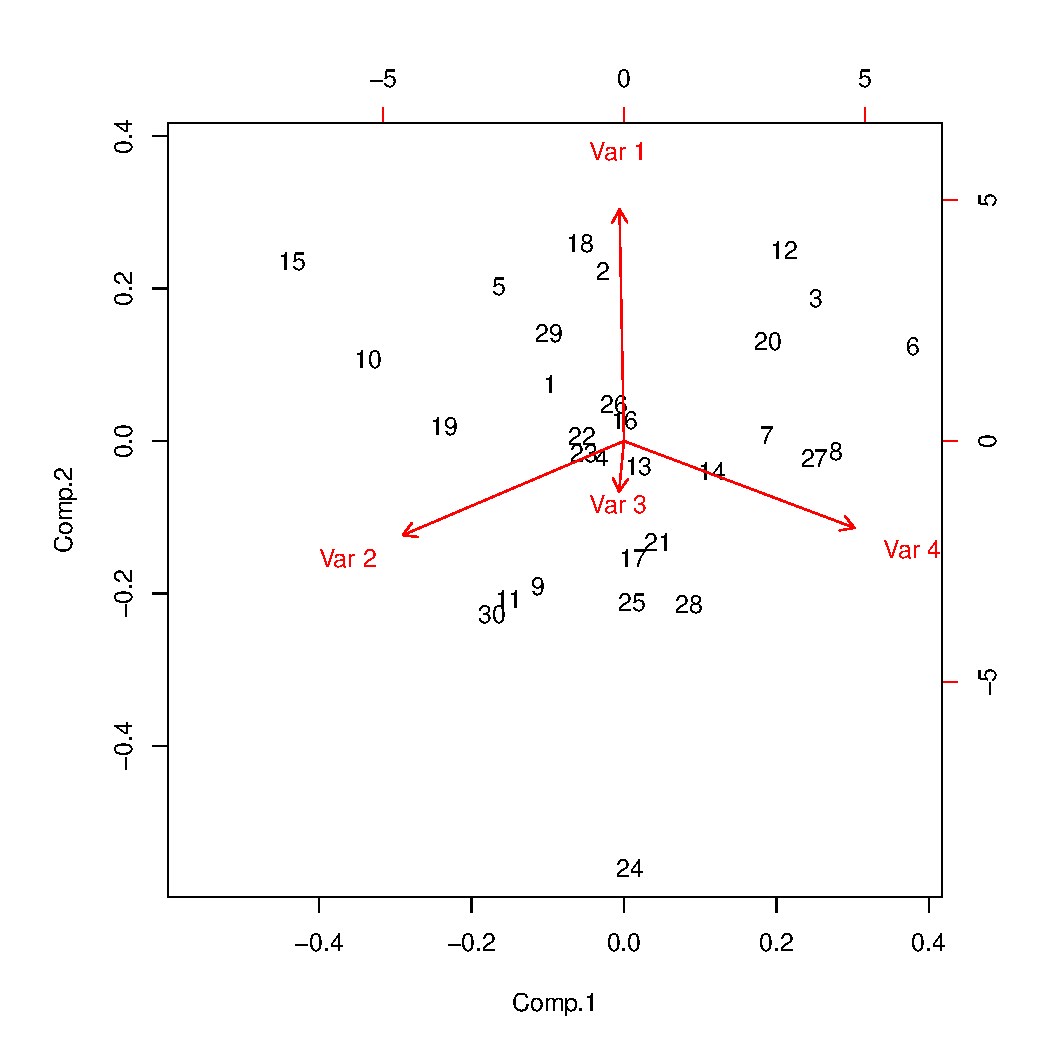
\includegraphics[width=\maxwidth]{figure/unnamed-chunk-6-1} 

\end{knitrout}

\section{Other}
\begin{enumerate}
\item Test for normality as follows:
\begin{knitrout}
\definecolor{shadecolor}{rgb}{0.969, 0.969, 0.969}\color{fgcolor}\begin{kframe}
\begin{alltt}
\hlcom{## This chunk was last ran in}
\hlkwd{timestamp}\hlstd{()}
\end{alltt}
\begin{verbatim}
## ##------ Thu Oct 25 12:14:21 2018 ------##
\end{verbatim}
\begin{alltt}
\hlkwd{data}\hlstd{(two_normal_pops)}
\hlkwd{par}\hlstd{(}\hlkwc{mfrow}\hlstd{=}\hlkwd{c}\hlstd{(}\hlnum{1}\hlstd{,}\hlnum{2}\hlstd{))}
\hlkwd{qqnorm.acomp}\hlstd{(}\hlkwd{acomp}\hlstd{(two_normal_pops}\hlopt{@}\hlkwc{count_matrix}\hlstd{),} \hlkwc{pch}\hlstd{=}\hlnum{19}\hlstd{,} \hlkwc{cex}\hlstd{=}\hlnum{0.2}\hlstd{)}
\end{alltt}
\end{kframe}
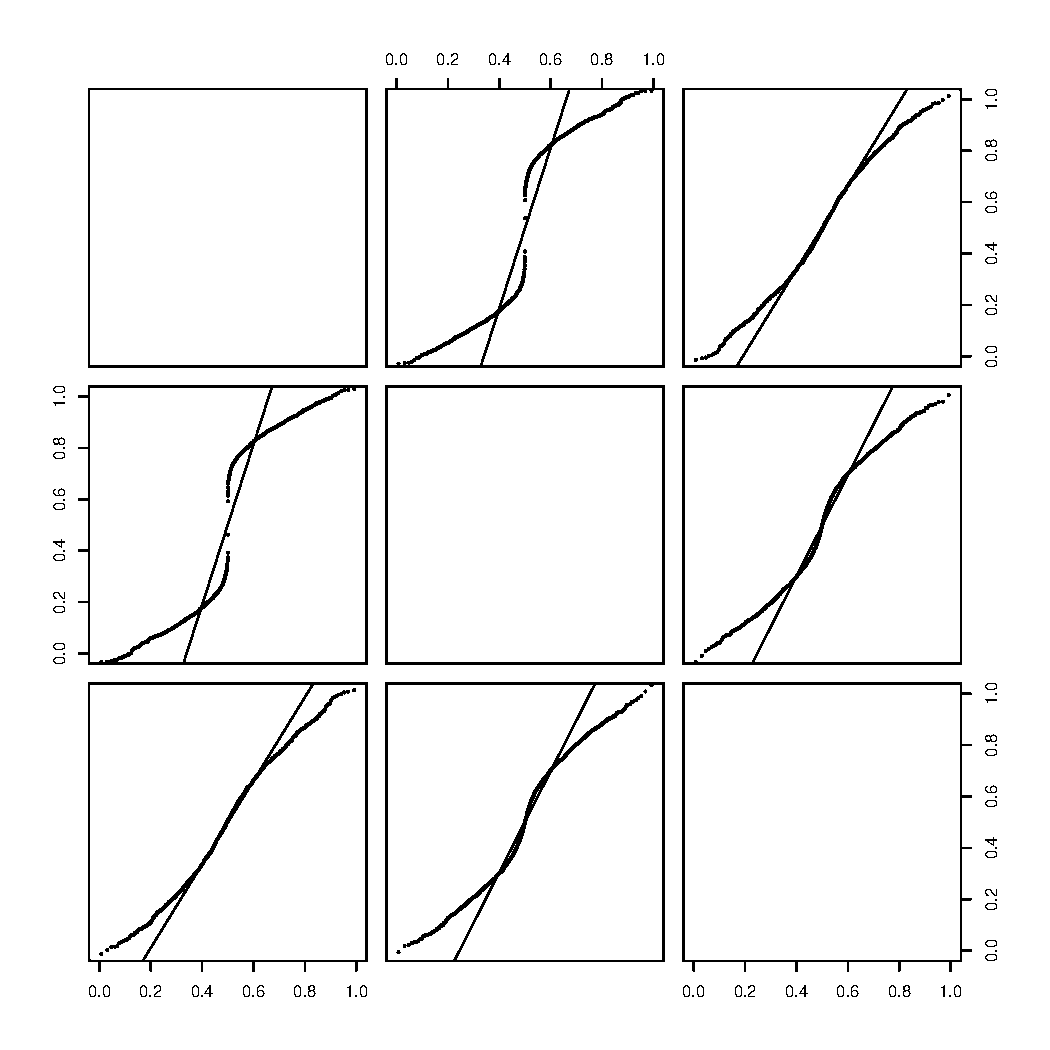
\includegraphics[width=\maxwidth]{figure/unnamed-chunk-7-1} 
\begin{kframe}\begin{alltt}
\hlkwd{qqnorm.acomp}\hlstd{(}\hlkwd{acomp}\hlstd{(two_normal_pops}\hlopt{@}\hlkwc{count_matrix}\hlstd{[}\hlnum{1}\hlopt{:}\hlnum{1000}\hlstd{,]),} \hlkwc{pch}\hlstd{=}\hlnum{19}\hlstd{,} \hlkwc{cex}\hlstd{=}\hlnum{0.2}\hlstd{,} \hlkwc{plot.it}\hlstd{=}\hlnum{FALSE}\hlstd{)}
\end{alltt}


{\ttfamily\noindent\color{warningcolor}{\#\# Warning in plot.window(...): "{}plot.it"{} is not a graphical parameter}}

{\ttfamily\noindent\color{warningcolor}{\#\# Warning in plot.xy(xy, type, ...): "{}plot.it"{} is not a graphical parameter}}

{\ttfamily\noindent\color{warningcolor}{\#\# Warning in title(...): "{}plot.it"{} is not a graphical parameter}}

{\ttfamily\noindent\color{warningcolor}{\#\# Warning in plot.window(...): "{}plot.it"{} is not a graphical parameter}}

{\ttfamily\noindent\color{warningcolor}{\#\# Warning in plot.xy(xy, type, ...): "{}plot.it"{} is not a graphical parameter}}

{\ttfamily\noindent\color{warningcolor}{\#\# Warning in title(...): "{}plot.it"{} is not a graphical parameter}}

{\ttfamily\noindent\color{warningcolor}{\#\# Warning in axis(side = side, at = at, labels = labels, ...): "{}plot.it"{} is not a graphical parameter}}

{\ttfamily\noindent\color{warningcolor}{\#\# Warning in plot.xy(xy.coords(x, y), type = type, ...): "{}plot.it"{} is not a graphical parameter}}

{\ttfamily\noindent\color{warningcolor}{\#\# Warning in plot.window(...): "{}plot.it"{} is not a graphical parameter}}

{\ttfamily\noindent\color{warningcolor}{\#\# Warning in plot.xy(xy, type, ...): "{}plot.it"{} is not a graphical parameter}}

{\ttfamily\noindent\color{warningcolor}{\#\# Warning in title(...): "{}plot.it"{} is not a graphical parameter}}

{\ttfamily\noindent\color{warningcolor}{\#\# Warning in axis(side = side, at = at, labels = labels, ...): "{}plot.it"{} is not a graphical parameter}}

{\ttfamily\noindent\color{warningcolor}{\#\# Warning in plot.xy(xy.coords(x, y), type = type, ...): "{}plot.it"{} is not a graphical parameter}}

{\ttfamily\noindent\color{warningcolor}{\#\# Warning in plot.window(...): "{}plot.it"{} is not a graphical parameter}}

{\ttfamily\noindent\color{warningcolor}{\#\# Warning in plot.xy(xy, type, ...): "{}plot.it"{} is not a graphical parameter}}

{\ttfamily\noindent\color{warningcolor}{\#\# Warning in title(...): "{}plot.it"{} is not a graphical parameter}}

{\ttfamily\noindent\color{warningcolor}{\#\# Warning in axis(side = side, at = at, labels = labels, ...): "{}plot.it"{} is not a graphical parameter}}

{\ttfamily\noindent\color{warningcolor}{\#\# Warning in plot.xy(xy.coords(x, y), type = type, ...): "{}plot.it"{} is not a graphical parameter}}

{\ttfamily\noindent\color{warningcolor}{\#\# Warning in plot.window(...): "{}plot.it"{} is not a graphical parameter}}

{\ttfamily\noindent\color{warningcolor}{\#\# Warning in plot.xy(xy, type, ...): "{}plot.it"{} is not a graphical parameter}}

{\ttfamily\noindent\color{warningcolor}{\#\# Warning in title(...): "{}plot.it"{} is not a graphical parameter}}

{\ttfamily\noindent\color{warningcolor}{\#\# Warning in plot.window(...): "{}plot.it"{} is not a graphical parameter}}

{\ttfamily\noindent\color{warningcolor}{\#\# Warning in plot.xy(xy, type, ...): "{}plot.it"{} is not a graphical parameter}}

{\ttfamily\noindent\color{warningcolor}{\#\# Warning in title(...): "{}plot.it"{} is not a graphical parameter}}

{\ttfamily\noindent\color{warningcolor}{\#\# Warning in plot.xy(xy.coords(x, y), type = type, ...): "{}plot.it"{} is not a graphical parameter}}

{\ttfamily\noindent\color{warningcolor}{\#\# Warning in plot.window(...): "{}plot.it"{} is not a graphical parameter}}

{\ttfamily\noindent\color{warningcolor}{\#\# Warning in plot.xy(xy, type, ...): "{}plot.it"{} is not a graphical parameter}}

{\ttfamily\noindent\color{warningcolor}{\#\# Warning in title(...): "{}plot.it"{} is not a graphical parameter}}

{\ttfamily\noindent\color{warningcolor}{\#\# Warning in axis(side = side, at = at, labels = labels, ...): "{}plot.it"{} is not a graphical parameter}}

{\ttfamily\noindent\color{warningcolor}{\#\# Warning in plot.xy(xy.coords(x, y), type = type, ...): "{}plot.it"{} is not a graphical parameter}}

{\ttfamily\noindent\color{warningcolor}{\#\# Warning in plot.window(...): "{}plot.it"{} is not a graphical parameter}}

{\ttfamily\noindent\color{warningcolor}{\#\# Warning in plot.xy(xy, type, ...): "{}plot.it"{} is not a graphical parameter}}

{\ttfamily\noindent\color{warningcolor}{\#\# Warning in title(...): "{}plot.it"{} is not a graphical parameter}}

{\ttfamily\noindent\color{warningcolor}{\#\# Warning in plot.xy(xy.coords(x, y), type = type, ...): "{}plot.it"{} is not a graphical parameter}}

{\ttfamily\noindent\color{warningcolor}{\#\# Warning in plot.window(...): "{}plot.it"{} is not a graphical parameter}}

{\ttfamily\noindent\color{warningcolor}{\#\# Warning in plot.xy(xy, type, ...): "{}plot.it"{} is not a graphical parameter}}

{\ttfamily\noindent\color{warningcolor}{\#\# Warning in title(...): "{}plot.it"{} is not a graphical parameter}}

{\ttfamily\noindent\color{warningcolor}{\#\# Warning in axis(side = side, at = at, labels = labels, ...): "{}plot.it"{} is not a graphical parameter}}

{\ttfamily\noindent\color{warningcolor}{\#\# Warning in axis(side = side, at = at, labels = labels, ...): "{}plot.it"{} is not a graphical parameter}}\end{kframe}
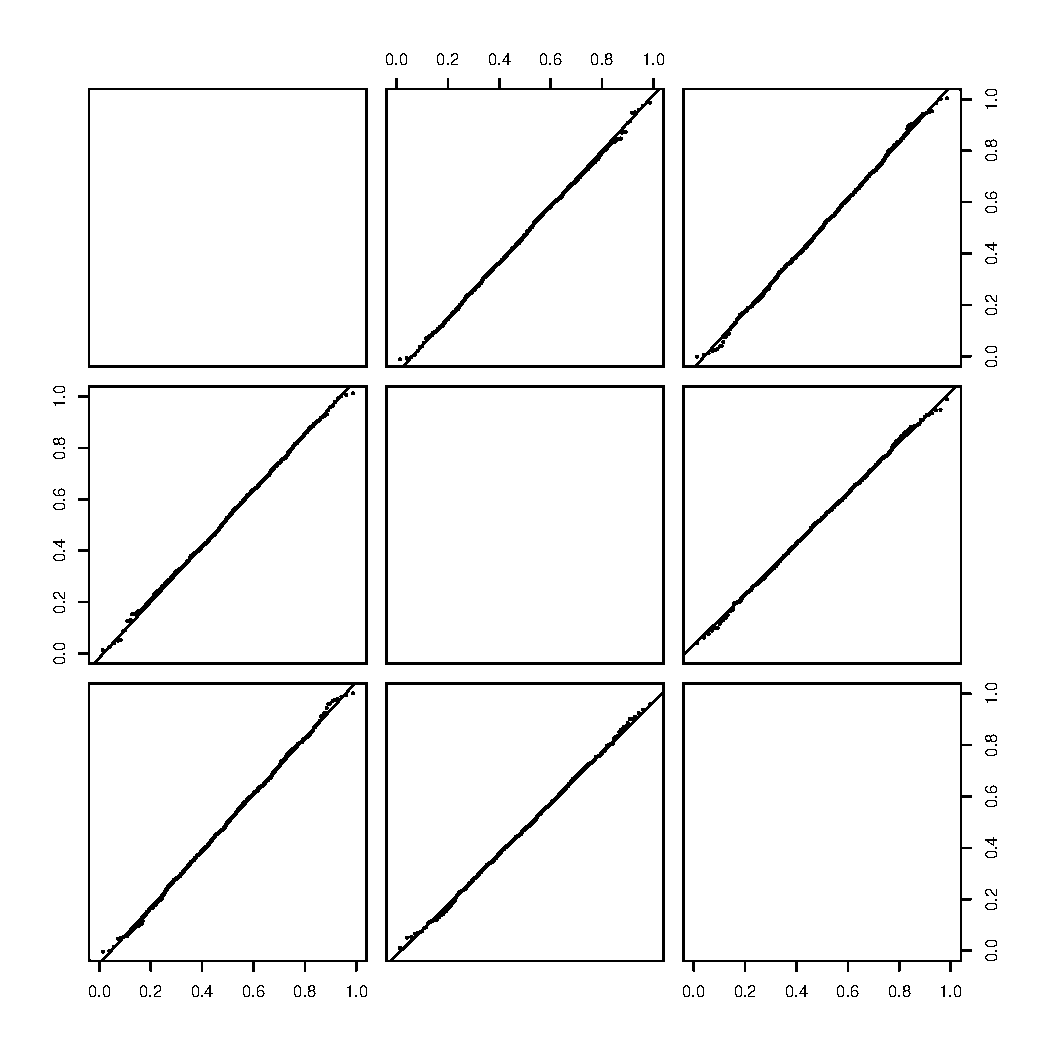
\includegraphics[width=\maxwidth]{figure/unnamed-chunk-7-2} 

\end{knitrout}
\end{enumerate}

\section{Clustering of samples}



\clearpage

\subsection{Testing hypotheses about two populations}
We might have our samples split into two categories; e.g. sex. As in Aithison 1986\cite{}, I follow a hierarchy of alternative hypotheses, from least to most complex.

Our first question is whether two populations have the same covariance and structure and center (i.e. if there is any distributional difference)

\begin{knitrout}
\definecolor{shadecolor}{rgb}{0.969, 0.969, 0.969}\color{fgcolor}\begin{kframe}
\begin{alltt}
\hlcom{## This chunk was last ran in}
\hlkwd{timestamp}\hlstd{()}
\end{alltt}
\begin{verbatim}
## ##------ Thu Oct 25 12:14:22 2018 ------##
\end{verbatim}
\begin{alltt}
\hlcom{##TODO!!}
\end{alltt}
\end{kframe}
\end{knitrout}

The next is whether the populations have a different center:

\begin{knitrout}
\definecolor{shadecolor}{rgb}{0.969, 0.969, 0.969}\color{fgcolor}\begin{kframe}
\begin{alltt}
\hlcom{## This chunk was last ran in}
\hlkwd{timestamp}\hlstd{()}
\end{alltt}
\begin{verbatim}
## ##------ Thu Oct 25 12:14:22 2018 ------##
\end{verbatim}
\begin{alltt}
\hlcom{## This dataset includes the two components above, as well as four others}
\hlcom{## (a total of seven)}
\hlkwd{data}\hlstd{(}\hlstr{"two_normal_pops_extended"}\hlstd{)}

\hlcom{## Data from the Landscape... paper}
\hlkwd{data}\hlstd{(}\hlstr{"Breast560"}\hlstd{)}

\hlstd{wrapper_compare_populations} \hlkwb{<-} \hlkwa{function}\hlstd{(}\hlkwc{predictors}\hlstd{,} \hlkwc{response}\hlstd{,} \hlkwc{...}\hlstd{)\{}
  \hlkwa{if}\hlstd{(}\hlkwd{length}\hlstd{(}\hlkwd{unique}\hlstd{(response))} \hlopt{==} \hlnum{2}\hlstd{)\{}
    \hlstd{tmp} \hlkwb{<-} \hlkwd{compare_populations}\hlstd{(predictors, response, ...)}
    \hlstd{tmp} \hlkwb{<-} \hlstd{tmp}\hlopt{$}\hlstd{info[}\hlnum{1}\hlopt{:}\hlnum{2}\hlstd{]}
    \hlstd{tmp}
  \hlstd{\}}
\hlstd{\}}

\hlstd{x} \hlkwb{<-} \hlkwd{do.call}\hlstd{(}\hlstr{'rbind'}\hlstd{,} \hlkwd{lapply}\hlstd{(}\hlnum{1}\hlopt{:}\hlkwd{ncol}\hlstd{(}\hlkwd{metadata}\hlstd{(Breast560)),}
       \hlkwa{function}\hlstd{(}\hlkwc{k}\hlstd{)\{}
         \hlkwd{wrapper_compare_populations}\hlstd{(}\hlkwc{predictors} \hlstd{=} \hlkwd{count_matrix}\hlstd{(Breast560),}
                                     \hlkwc{response} \hlstd{=} \hlkwd{metadata}\hlstd{(Breast560)[,k])}
         \hlstd{\}}
       \hlstd{))}


\hlstd{x}
\end{alltt}
\begin{verbatim}
##          test      p-value
## [1,] 223.6681 6.334800e-26
## [2,] 237.6260 6.270514e-29
## [3,] 237.4362 2.457445e-43
## [4,]  78.3811 9.584122e-12
\end{verbatim}
\end{kframe}
\end{knitrout}


\section{Data for 560 breast cancer patients}
Data from 560 breast cancer patients is available as part of the document as well:

\begin{knitrout}
\definecolor{shadecolor}{rgb}{0.969, 0.969, 0.969}\color{fgcolor}\begin{kframe}
\begin{alltt}
\hlcom{#data("Breast560")}
\hlcom{#metadata(Breast560)[1:4,1:5]}
\hlcom{#count_matrix(Breast560)[1:4,1:5]}
\end{alltt}
\end{kframe}
\end{knitrout}


\section{Data for 12k TCGA samples, with ovarian cancer-derived CNA signatures}



